\hypertarget{ux63a7ux5236ux5c0fux8f66}{%
\subsection{控制小车}\label{ux63a7ux5236ux5c0fux8f66}}

上一节我们已经搭好了开发环境,接下来就可以写 Python
程序来控制小车了。首先用 EV3
主机、大型伺服马达和超声波传感器搭建一个小车:

 
 \begin{figure}[htp]
	\centering
	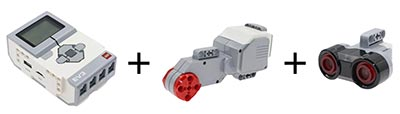
\includegraphics[width=0.6\linewidth]{fig/1346290325651521l.png}
\end{figure}


可以自由发挥,我的小车完成后长这样:

 
 \begin{figure}[htp]
	\centering
	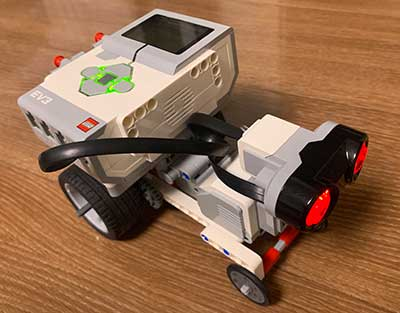
\includegraphics[width=0.6\linewidth]{fig/1346290294194241l.png}
\end{figure}


下一步,我们用程序控制小车。首先根据马达和传感器接入的位置初始化如下:

\begin{pythoncode}
motor = Motor(Port.B) # 接在B口
ultrasonic = UltrasonicSensor(Port.S4) # 接在4号口
\end{pythoncode}

然后,设置初始速度 0 表示静止:

\begin{pythoncode}
speed = 0
\end{pythoncode}

通过传入\texttt{1}、\texttt{-1}和\texttt{0}分别表示加速、减速和停止:

\begin{pythoncode}
def setSpeed(acc):
    global speed
    if acc < 0:
        speed = max(0, speed - 1)
    elif acc > 0:
        speed = min(3, speed + 1)
    else:
        speed = 0
    if speed > 0:
        motor.run(speed * 90) 
    else:
        motor.stop()
\end{pythoncode}

因为小车的初始速度为
0,我们可以设定响应右键加速,左键减速,中键停止,上键停止并退出,用一个无限循环实现功能如下:

\begin{pythoncode}
while True:
    if not any(brick.buttons()): 
        wait(10)
    else:
        if Button.LEFT in brick.buttons():
            setSpeed(-1)
        elif Button.RIGHT in brick.buttons():
            setSpeed(1)
        elif Button.CENTER in brick.buttons():
            setSpeed(0)
        elif Button.UP in brick.buttons():
            setSpeed(0)
            break
        wait(500)
    if ultrasonic.distance() < 200: 
        setSpeed(0)
\end{pythoncode}

因为 EV3 的控制 API
并没有提供回调,所以只能通过无限循环主动轮询。使用无限循环时需要注意,务必在每次循环内部通过\texttt{wait()}暂停若干毫秒,否则很容易耗尽
CPU。最后,我们通过超声波传感器返回的距离判断是否自动停车。

加上声光特效后,来看看实际效果:

EV3 的 Python 接口全部在\texttt{pybricks}包中,要查看完整的 API,请在 VS
Code 新建 EV3 工程时选择 ``Open user guide and
examples'',即可在本地浏览器打开 API 文档。

\hypertarget{ux53c2ux8003ux6e90ux7801}{%
\subsubsection{参考源码}\label{ux53c2ux8003ux6e90ux7801}}

\href{https://github.com/michaelliao/learn-python3/tree/master/samples/micropython/smallcar}{smallcar}

